\special{dvipdfmx:config z 0}
\documentclass{article}
\usepackage{marcythm}

\title{Undergraduate Complexity Theory \\ Lecture 3: Simulation and Turing Machine Variants}
\author{Marcythm}
% \date{\today}
\date{July 9, 2022}

\begin{document}
\maketitle{}

\section{Lecture Notes}

Somethings we are going to prove or talk about today:

\begin{figure}[h]
  \begin{tikzpicture}
    \node [ellipse, draw=black] (TM) at (0, 0) {1-tape TM};

    % \node [ellipse, draw=black] (1wayTM) at (-2, 1.5) {(1-tape, 1-way inf) TM};
    \node [ellipse, draw=black] (1wayTM) at (0, 2.5) {(1-tape, 1-way inf) TM};
    \draw [->] (TM) edge[right, bend right] node{\(T\)} (1wayTM);
    \draw [->] (1wayTM) edge[left, bend right] node{\(T\)} (TM);

    % \node [ellipse, draw=black, align=center] (3alphTM) at (-2, -1.5) {1-tape TM \\ \(\Gamma = \braces{0, 1, b}\)};
    \node [ellipse, draw=black, align=center] (3alphTM) at (-4, 0) {1-tape TM \\ \(\Gamma = \braces{0, 1, b}\)};
    \draw [->] (TM) edge[above, bend right] node{\(T\)} (3alphTM);
    \draw [->] (3alphTM) edge[above, bend right] node{\(T\)} (TM);

    \node [ellipse, draw=black] (multiTM) at (4, 0) {multitape TM};
    \draw [->] (TM) edge[above, bend right] node{\(T\)} (multiTM);
    \draw [->] (multiTM) edge[above, bend right] node{\(T^2\)} (TM);

    \node [ellipse, draw=black, align=center] (RAM) at (9, 0) {C-like pesudocode \\ RAM model};
    \draw [->] (multiTM) edge[above, bend right] node{\(T \log T\)} (RAM);
    \draw [->] (RAM) edge[above, bend right] node{\(T^2\)} (multiTM);

    \node [ellipse, draw=black, align=center] (BooleanCircuit) at (0, -3) {Boolean \\ Circuit};
    \draw [->] (TM) edge[left, bend right] node{\(T \log T\)} (BooleanCircuit);
    \draw [->] (BooleanCircuit) edge[right, bend right, dashed] node[align=center]{non-uniformity \\ (give a different algo \\ for every input length)} (TM);
  \end{tikzpicture}
\end{figure}

\begin{definition}
  \resizebox{!}{\height}{
    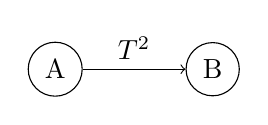
\begin{tikzpicture}
      \node [shape=circle, draw=black] (A) at (0,0) {A};
      \node [shape=circle, draw=black] (B) at (2,0) {B};

      \draw [->] (A) edge[above] node{\(T^2\)} (B);
    \end{tikzpicture}
  }
  means can ``compile'' (simulate) code \(M_A\) in model \(A\) to code \(M_B\) in model \(B\), s.t.\ if \(M_A\) runs in time \(T\), then \(M_B\) runs in time \(O(T^2)\).
\end{definition}

\begin{definition}
  For a {\bf decider} \(M\), the {\it running time (time complexity)} of \(M\) is a function \(T: \N \to \N\):
  \[ T(n) = \max_{\abs{x} = n} \braces{\text{\# steps \(M(x)\) takes}} \]
\end{definition}

\begin{remark}
  Time Complexity is a {\bf function} of \(n\), because we care about how it {\bf scales} with input size.
\end{remark}

TM tricks:
\begin{enumerate}
  \item Allow TMs to `S'tay and put in a step besides L/R.
  \item LL/RR in the same way.
  \item ``Marking'' a cell. Impl: just double the tape alphabet \(\Gamma\). \\
        Simulate 2-way infinite TM with 1-way infinite TM: using marking trick to indicate left boundary.
  \item ``Stretching'' an input, i.e. \(abcc \to a\_b\_c\_c\). \\
        Simulate \(\Gamma = \setof{0, 1, b, \dot{0}, \dot{1}, \dot{b}, \#}\) with \(\Gamma = \setof{0, 1, b}\): use stretch to have room for new encoding. \\
        Simulate multitape TM with 1-tape TM.
\end{enumerate}

\section{Reading}

\subsection{Sipser 3.2 (Variants of Turing Machines)}

\begin{enumerate}
  \item multitape TM, and how to simulate it
\end{enumerate}

\subsection{Sipser 7.1 (Measuring Complexity)}

\begin{enumerate}
  \item time complexity of TM
  \item asymptotic notations
  \item difference between:
  \begin{enumerate}
    \item computability theory: all reasonable models of computation are equivalent, i.e.\ they all decide the same class of languages.
    \item complexity theory: the choice of model affects the time complexity of languages.
  \end{enumerate}
\end{enumerate}

\end{document}
